\documentclass[../main.tex]{subfiles}
\begin{document}
Omdat smartwatch apps gebruiksonvriendelijker worden na mate ze ingewikkeld worden, staat eenvoud bovenop. Daarnaast moeten de lopers vooral bezig zijn met lopen, en zijn de andere activiteiten omheen de verantwoordelijkheid voor de andere teamleden.
Wij hebben daarom besloten om 2 schermen te gebruiken. Op het eerste scherm worden de actuele data weergegeven, d.w.z. hartslag, aantal gelopen stappen, en huidige snelheid.

Op het tweede scherm wordt de huidige locatie weergegeven op Google Maps, met een pad met de gelopen route en een projectie van de nog te lopen route. Dit is puur als indicatie bedoeld, omdat de navigatie door de fietsende begeleiders gedaan wordt.

Alle informatie, d.w.z. biometrische gegeven, locatie, hoogteverschillen etc. worden op een server opgeslagen. Later kunnen wij de data samenvoegen tot een mooi, overzichtelijk geheel van alle statistieken, waardes per gelopen stuk, gemiddelde waardes per dag en per evenement, en mooie grafieken. De informatie kunnen dan gedeeld worden met vrienden, familie en supporters.

\begin{figure}[h]
    \centering
	\caption{Applicatie demo}
    \label{fig:demo}
    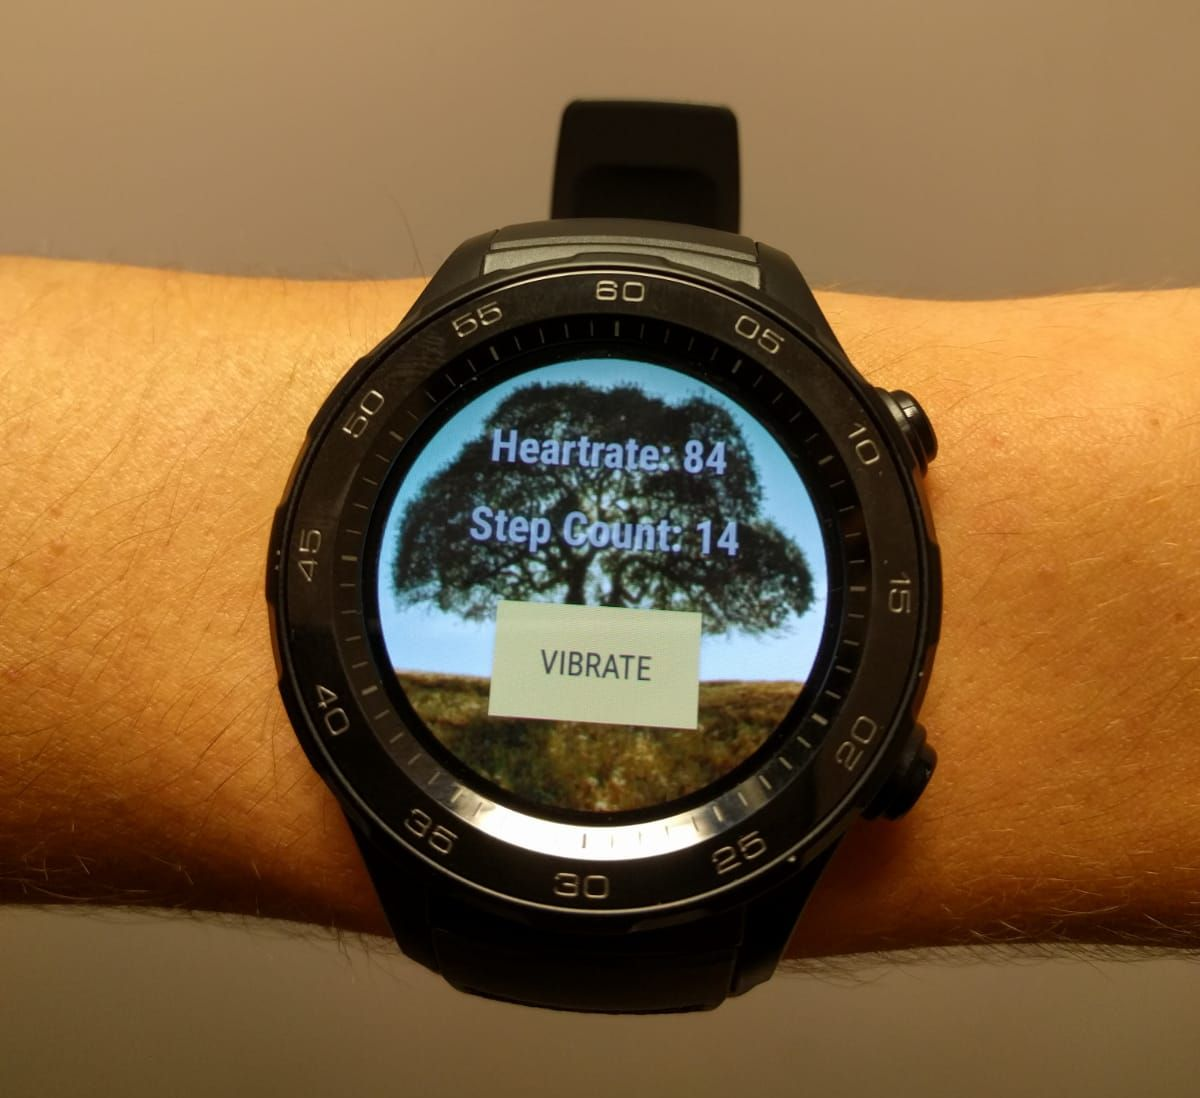
\includegraphics[width=110mm]{demo.jpg}
\end{figure}

\end{document}
